\chapter{Lampiran A. Tangkapan Layar Hasil Pengujian Regresi}
\label{lampiran_a}

\begin{figure}[!htb]
	\centering
	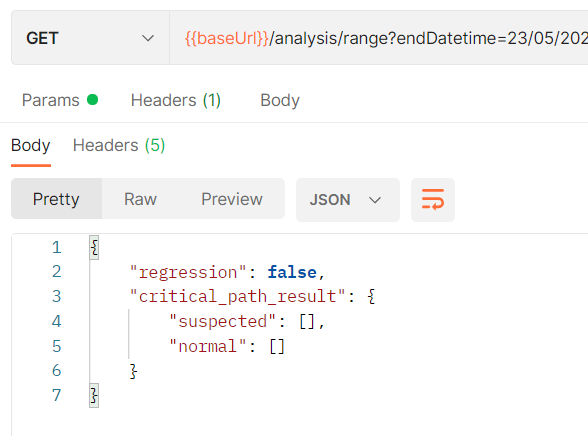
\includegraphics[width=0.75\textwidth]{resources/ch4/json/1-new.png}
	\caption{\textit{Response} JSON hasil pengujian kasus \textbf{SI1}}
	\label{result_json_1}
\end{figure}

%\begin{figure}[!htb]
%	\centering
%	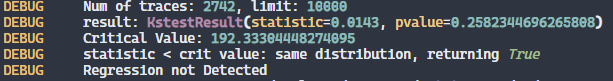
\includegraphics[width=1\textwidth]{resources/ch4/log/1-log.png}
%	\caption{\textit{Log} hasil pengujian kasus SI1}
%	\label{result_log_1}
%\end{figure}

\begin{figure}[!htb]
	\centering
	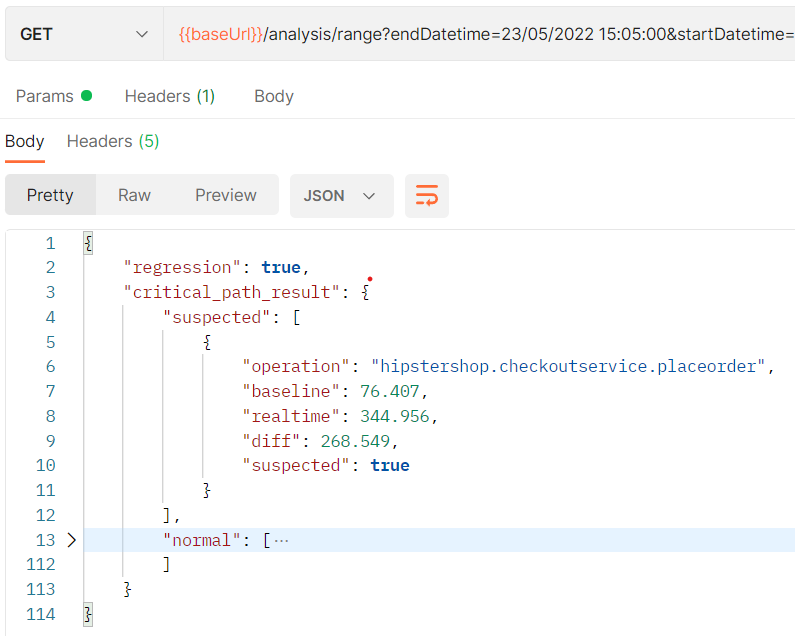
\includegraphics[width=0.75\textwidth]{resources/ch4/json/2-new.png}
	\caption{\textit{Response} JSON hasil pengujian kasus \textbf{SI2}}
	\label{result_json_2}
\end{figure}

%\begin{figure}[!htb]
%	\centering
%	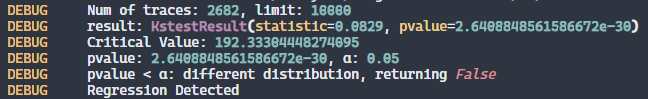
\includegraphics[width=1\textwidth]{resources/ch4/log/2-log.png}
%	\caption{\textit{Log} hasil pengujian kasus SI2}
%	\label{result_log_2}
%\end{figure}

\begin{figure}[!htb]
	\centering
	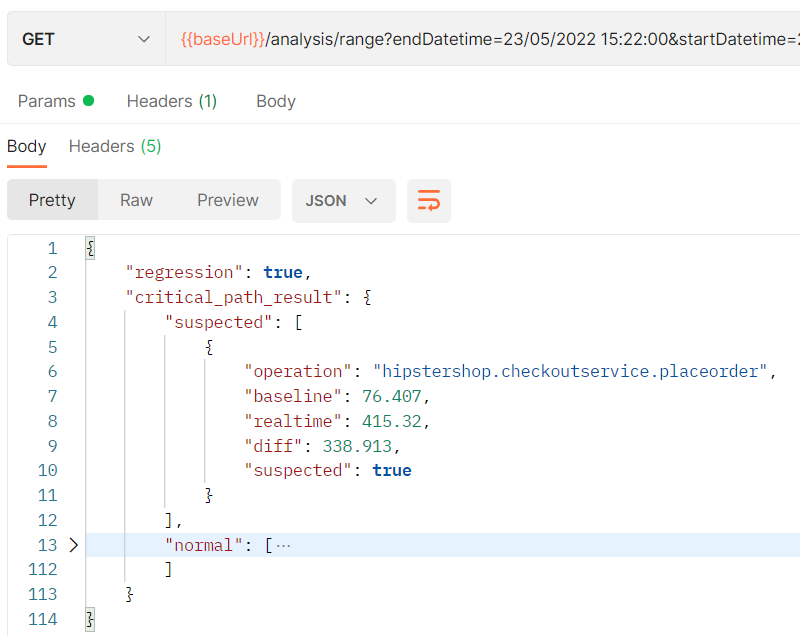
\includegraphics[width=0.75\textwidth]{resources/ch4/json/3-new.png}
	\caption{\textit{Response} JSON hasil pengujian kasus \textbf{SI3}}
	\label{result_json_3}
\end{figure}

%\begin{figure}[!htb]
%	\centering
%	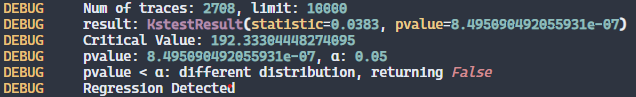
\includegraphics[width=1\textwidth]{resources/ch4/log/3-log.png}
%	\caption{\textit{Log} hasil pengujian kasus SI3}
%	\label{result_log_3}
%\end{figure}
%\pagebreak

\begin{figure}[!htb]
	\centering
	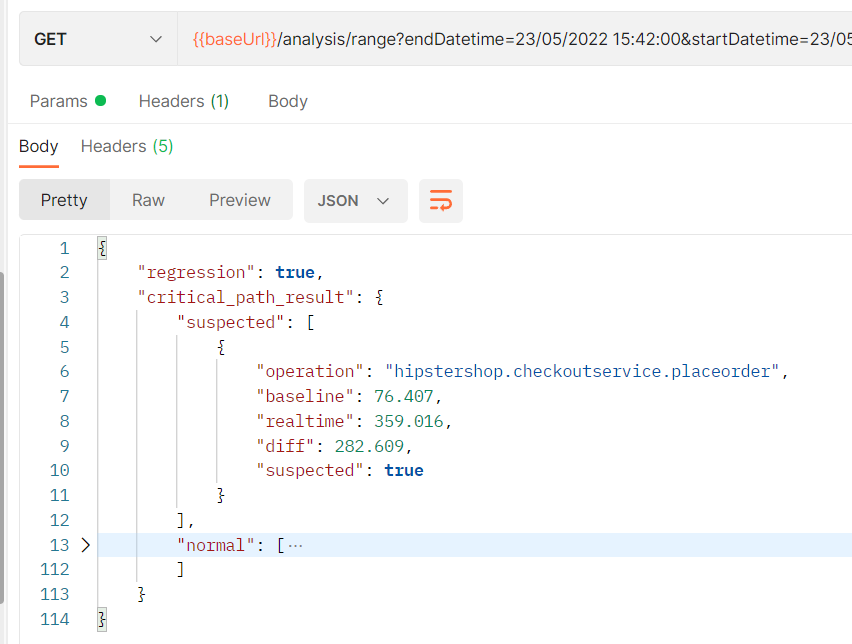
\includegraphics[width=0.75\textwidth]{resources/ch4/json/4-new.png}
	\caption{\textit{Response} JSON hasil pengujian kasus \textbf{SI4}}
	\label{result_json_4}
\end{figure}

%\begin{figure}[!htb]
%	\centering
%	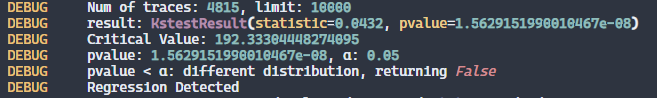
\includegraphics[width=1\textwidth]{resources/ch4/log/4-log.png}
%	\caption{\textit{Log} hasil pengujian kasus SI4}
%	\label{result_log_4}
%\end{figure}

\begin{figure}[!htb]
	\centering
	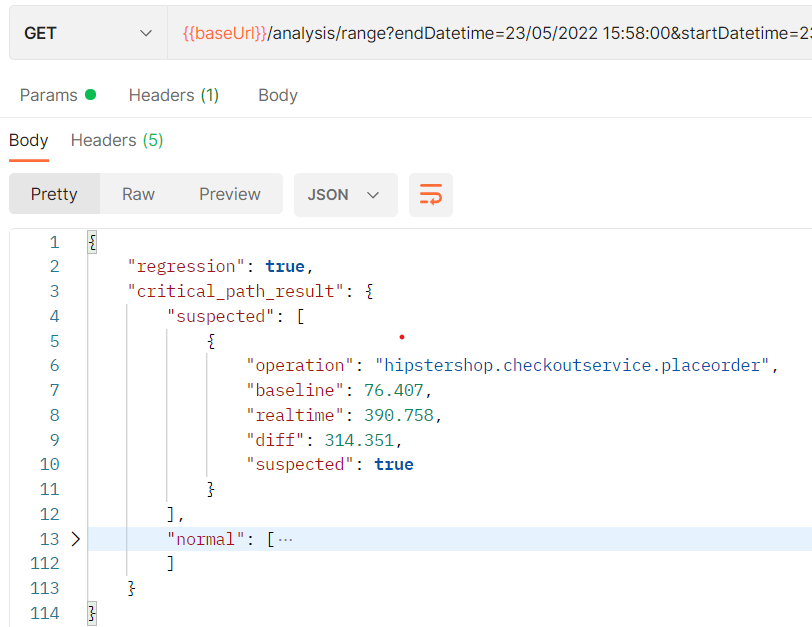
\includegraphics[width=0.75\textwidth]{resources/ch4/json/5-new.png}
	\caption{\textit{Response} JSON hasil pengujian kasus \textbf{SI5}}
	\label{result_json_5}
\end{figure}

%\begin{figure}[!htb]
%	\centering
%	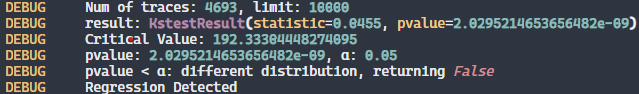
\includegraphics[width=1\textwidth]{resources/ch4/log/5-log.png}
%	\caption{\textit{Log} hasil pengujian kasus \textbf{SI5}}
%	\label{result_log_5}
%\end{figure}

\begin{figure}[!htb]
	\centering
	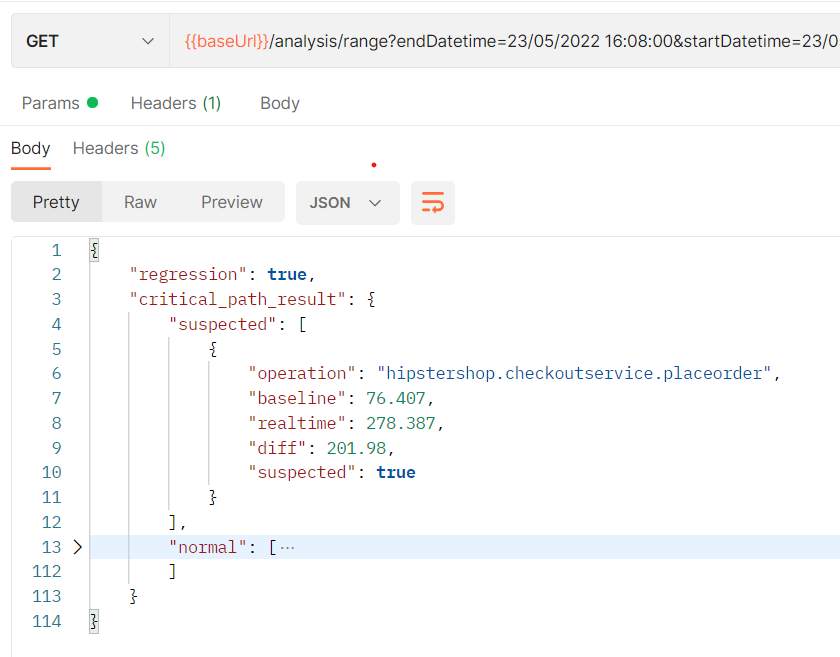
\includegraphics[width=0.75\textwidth]{resources/ch4/json/6-new.png}
	\caption{\textit{Response} JSON hasil pengujian kasus \textbf{SI6}}
	\label{result_json_6}
\end{figure}

%\begin{figure}[!htb]
%	\centering
%	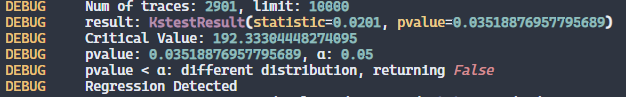
\includegraphics[width=1\textwidth]{resources/ch4/log/6-log.png}
%	\caption{\textit{Log} hasil pengujian kasus SI6}
%	\label{result_log_6}
%\end{figure}
%\pagebreak

\begin{figure}[!htb]
	\centering
	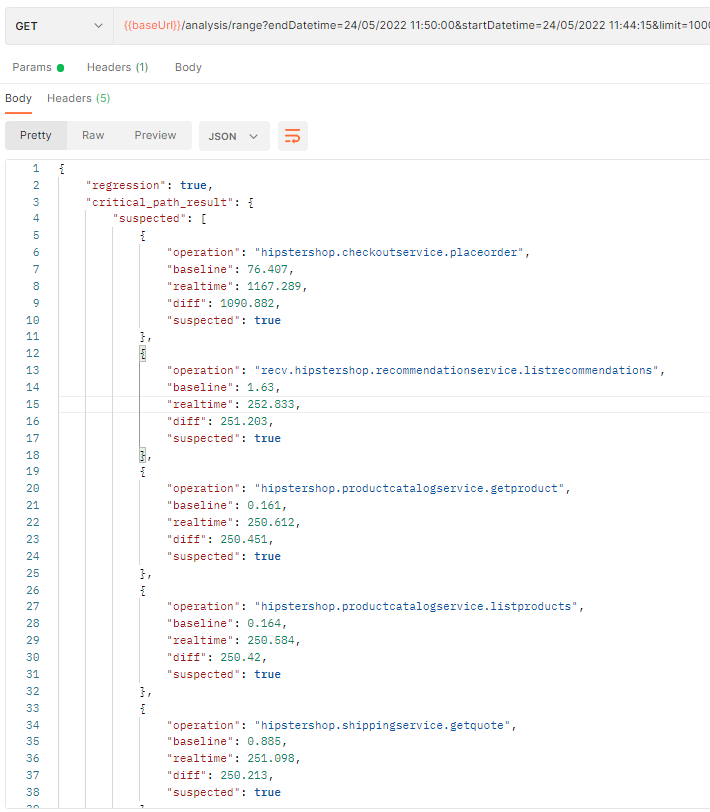
\includegraphics[width=0.75\textwidth]{resources/ch4/json/7-new.png}
	\caption{\textit{Response} JSON hasil pengujian kasus \textbf{SI7}}
	\label{result_json_7}
\end{figure}
%
%\begin{figure}[!htb]
%	\centering
%	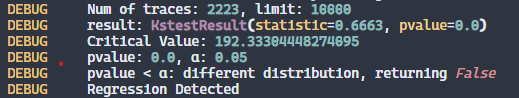
\includegraphics[width=1\textwidth]{resources/ch4/log/7-log.png}
%	\caption{\textit{Log} hasil pengujian kasus SI7}
%	\label{result_log_7}
%\end{figure}

\begin{figure}[!htb]
	\centering
	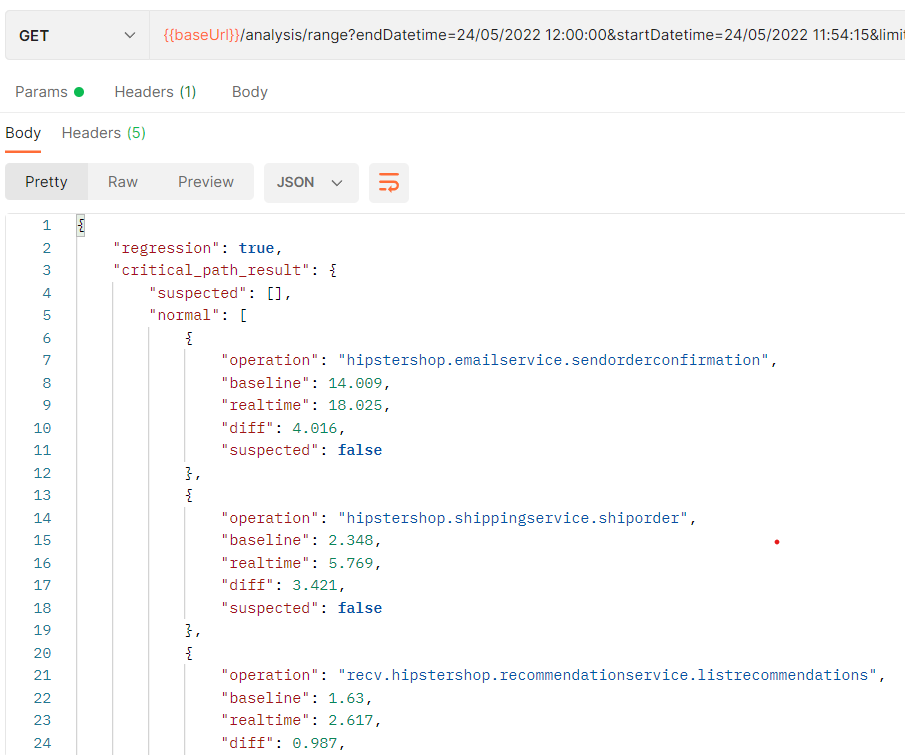
\includegraphics[width=0.75\textwidth]{resources/ch4/json/8-new.png}
	\caption{\textit{Response} JSON hasil pengujian kasus \textbf{SE1}}
	\label{result_json_8}
\end{figure}

%\begin{figure}[!htb]
%	\centering
%	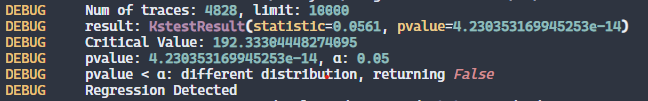
\includegraphics[width=1\textwidth]{resources/ch4/log/8-log.png}
%	\caption{\textit{Log} hasil pengujian kasus SE1}
%	\label{result_log_8}
%\end{figure}

\begin{figure}[!htb]
	\centering
	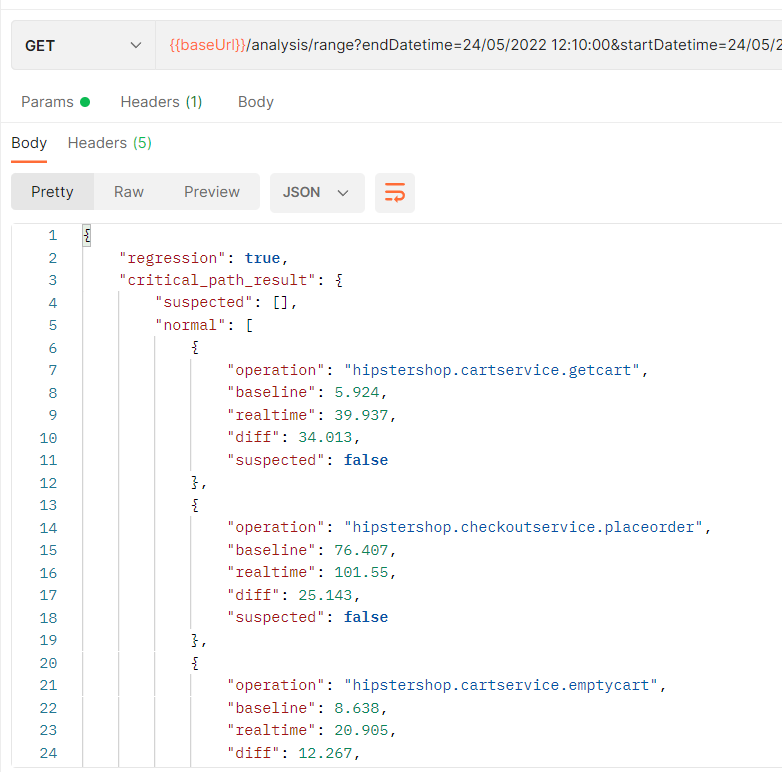
\includegraphics[width=0.75\textwidth]{resources/ch4/json/9-new.png}
	\caption{\textit{Response} JSON hasil pengujian kasus \textbf{SE2}}
	\label{result_json_9}
\end{figure}

%\begin{figure}[!htb]
%	\centering
%	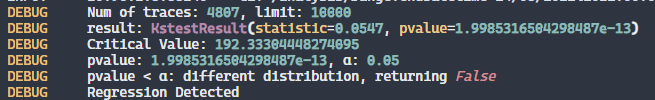
\includegraphics[width=1\textwidth]{resources/ch4/log/9-log.png}
%	\caption{\textit{Log} hasil pengujian kasus SE2}
%	\label{result_log_9}
%\end{figure}

\begin{figure}[!htb]
	\centering
	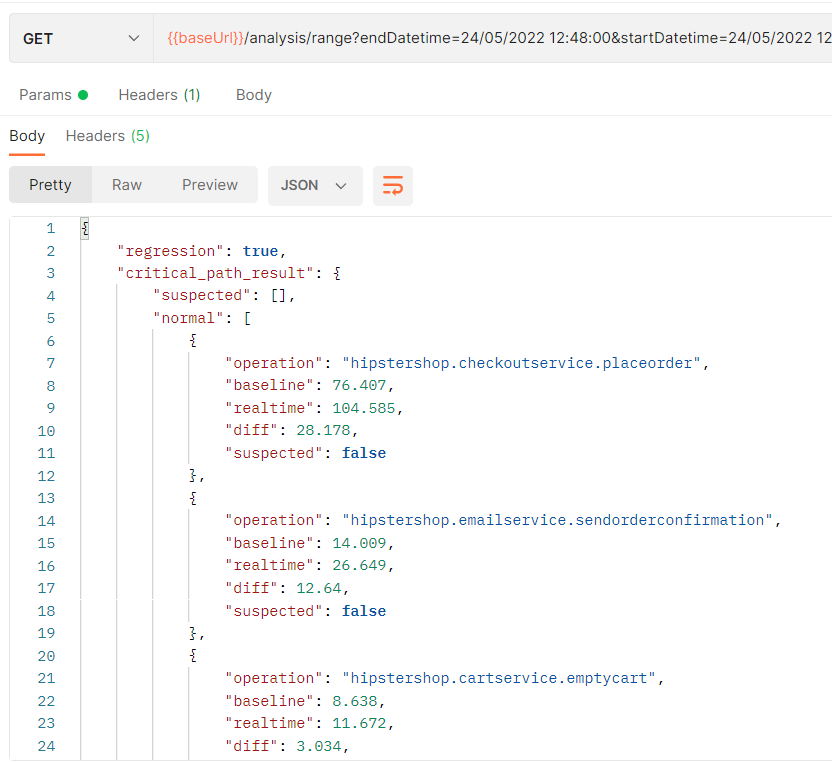
\includegraphics[width=0.75\textwidth]{resources/ch4/json/10-new.png}
	\caption{\textit{Response} JSON hasil pengujian kasus \textbf{SE3}}
	\label{result_json_10}
\end{figure}
%\begin{figure}[!htb]
%	\centering
%	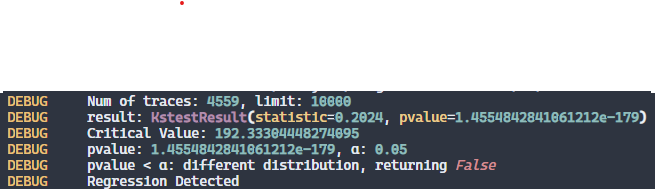
\includegraphics[width=1\textwidth]{resources/ch4/log/10-log.png}
%	\caption{\textit{Log} hasil pengujian kasus SE3}
%	\label{result_log_10}
%\end{figure}

\begin{figure}[!htb]
	\centering
	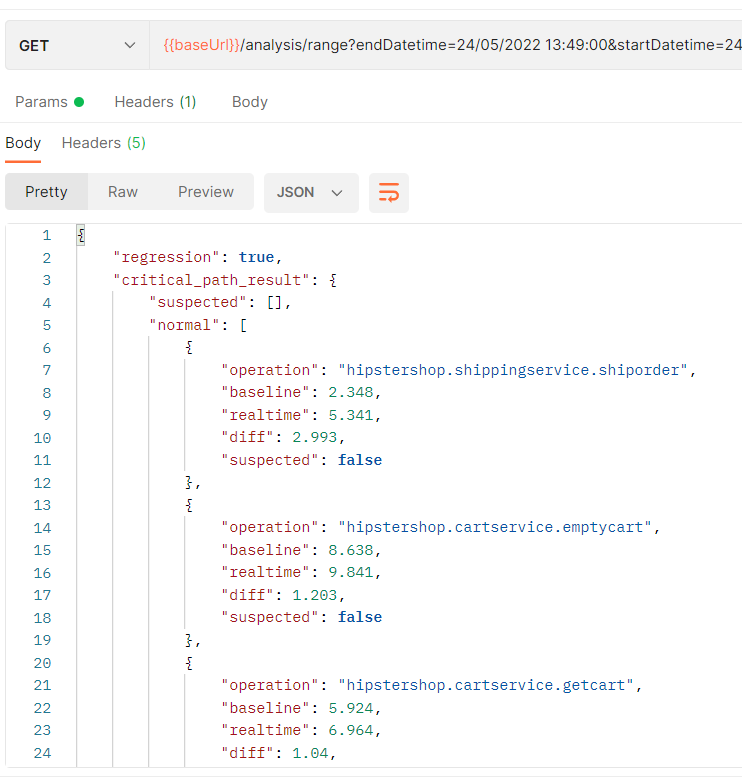
\includegraphics[width=0.75\textwidth]{resources/ch4/json/11-new.png}
	\caption{\textit{Response} JSON hasil pengujian kasus \textbf{SE4}}
	\label{result_json_11}
\end{figure}

%\begin{figure}[!htb]
%	\centering
%	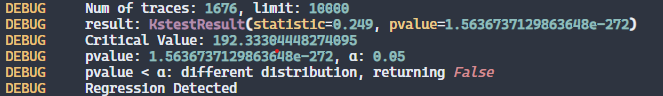
\includegraphics[width=1\textwidth]{resources/ch4/log/11-log.png}
%	\caption{\textit{Log} hasil pengujian kasus SE4}
%	\label{result_log_11}
%\end{figure}